\section{Spatial deformation and elapsed time}
\label{sec:geometry}
\subsection{Clock rates require the lapse}
For observers held at fixed spatial coordinates, Eq.~\eqref{eq:perturbed}
gives
\begin{equation}\label{eq:lapse}
 \dd\tau=\frac{A}{c}\sqrt{1+2\ph}\,\dd\eta
 =(1+\ph)\dd t+\order(\epsilon^2).
\end{equation}
A negative potential reduces the elapsed proper time relative to the
chosen background-time interval. To first order the accumulated change
at a fixed coordinate position is
\begin{equation}\label{eq:clock-offset}
 \delta\tau(\chi)=\frac{1}{c}\int_{\eta_1}^{\eta_2}
 A(\eta)\ph(\eta,\chi)\,\dd\eta.
\end{equation}
The normal observers used here need not follow the perturbed dust flow:
the latter has velocity from Eq.~\eqref{eq:constraint-velocity}.
Clock comparisons across separated worldlines require specified events
and a synchronization or signal protocol. Equation~\eqref{eq:clock-offset}
states explicitly which coordinate endpoints are being compared; it is
not a claim of an absolute local cosmic age.

\subsection{A spatial embedding has a different sign}
At fixed $\eta$, an approximate radial embedding in Euclidean four-space is
\begin{equation}\label{eq:deformed-embedding}
 \bm X(\eta,\bm n)=A(\eta)[1-\ph(\eta,\bm n)]\bm n.
\end{equation}
Because $\bm n\cdot\dd\bm n=0$, its induced line element is
\begin{align}
 \dd\bm X\cdot\dd\bm X
 &=A^2\left[(1-\ph)^2\dd\Omega_3^2+(\dd\ph)^2\right]\\
 &=A^2(1-2\ph)\dd\Omega_3^2+\order(\epsilon^2).
 \label{eq:induced}
\end{align}
Thus it reproduces the spatial metric to first order for a fixed smooth
profile as $\epsilon\to0$. Gradients must also be controlled: for narrow
profiles, discarded terms scale as $\epsilon^2/\sigma^2$ rather than
simply $\epsilon^2$ with a width-independent coefficient.

At the core $\ph<0$, Eq.~\eqref{eq:deformed-embedding} produces an
\emph{outward} deformation, while Eq.~\eqref{eq:lapse} produces slower
clocks. This is a result of this particular first-order spatial embedding
and time slicing; it is not a universal rule that mass must bulge outward
in every embedding diagram. It does show why the rubber-sheet ``dent''
cannot simultaneously be assumed to measure earlier cosmic time.

The intrinsic spatial-curvature perturbation provides another way to
describe the distortion:
\begin{equation}\label{eq:spatial-curvature}
 {}^{(3)}R=\frac{6}{A^2}
 +\frac{4}{A^2}(\nabla_\gamma^2+3)\ph+\order(\epsilon^2).
\end{equation}
It is the scalar curvature of the specified spatial slices. Its
perturbation, like the slices themselves, depends on the chosen slicing.
It is distinct from the extrinsic appearance of a curve on a page.

\begin{figure}[htbp]
 \centering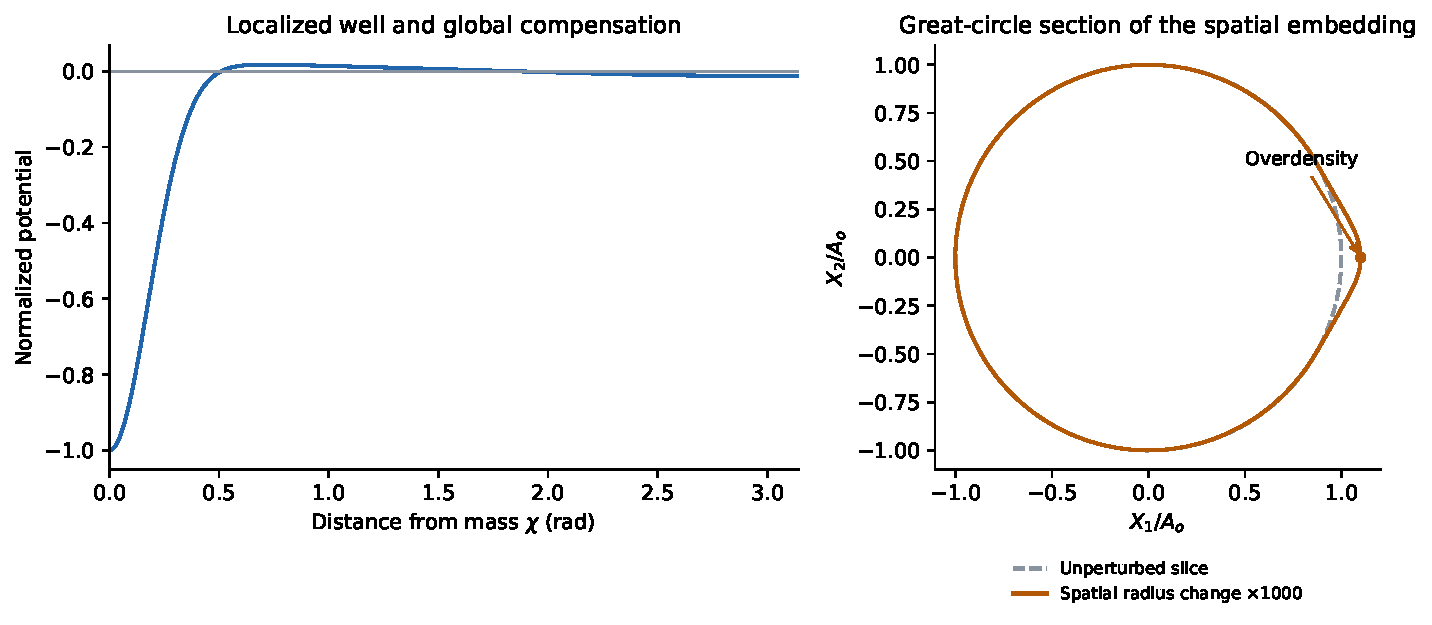
\includegraphics[width=\linewidth]{02-spatial-deformation.pdf}
 \caption{The potential profile at reception and a great-circle section
 of Eq.~\eqref{eq:deformed-embedding}. The plotted radial deformation is
 amplified by a factor of 1000 to make its sign visible. The amplified
 curve is illustrative, not an isometric embedding at the displayed
 amplitude. The physical fractional radius change at the core is $10^{-4}$.}
 \label{fig:deformation}
\end{figure}
\begin{figure}[htbp]
 \centering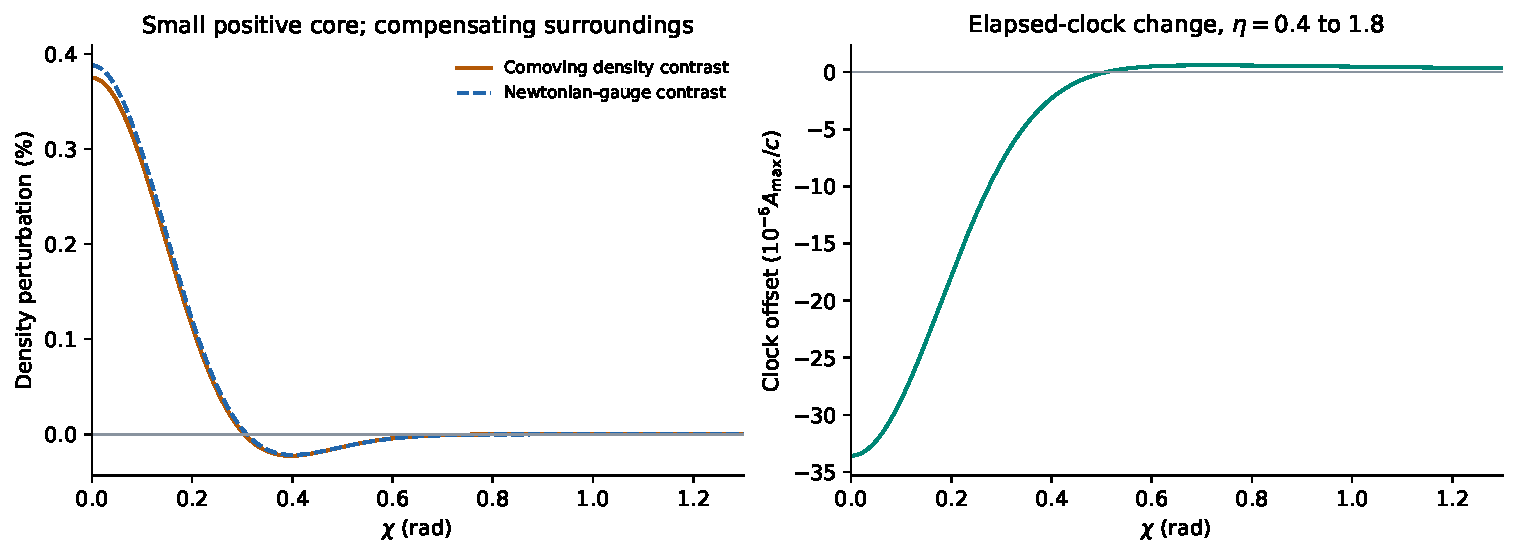
\includegraphics[width=\linewidth]{03-density-and-clocks.pdf}
 \caption{The density contrasts and the accumulated first-order
 normal-observer clock offset. Both follow from the same potential.
 The clock interval uses fixed background conformal times, and the
 surrounding density compensation is part of the model.}
 \label{fig:clocks}
\end{figure}
